\documentclass[12pt,letter]{article}
\usepackage{geometry}\geometry{top=0.75in}
\usepackage{amsmath}
\usepackage{amssymb}
\usepackage{mathtools}
\usepackage{xcolor} % Color words
\usepackage{cancel} % Crossing parts of equations out
\usepackage{tikz}       % Drawing 
\usetikzlibrary{shapes.geometric, arrows}
\usepackage{pgfplots}   % Other plotting
\usepgfplotslibrary{colormaps,fillbetween}
\usepackage{placeins}   % Float barrier

% Don't indent
\setlength{\parindent}{0pt}
% Function to replace \section with a problem name specifically formatted
\newcommand{\problem}[1]{\vspace{3mm}\Large\textbf{{Problem
{#1}\vspace{3mm}}}\normalsize\\}
% Formatting function, like \problem
\newcommand{\ppart}[1]{\vspace{2mm}\large\textbf{\\Part
{#1})\vspace{2mm}}\normalsize\\}
% Formatting 
\newcommand{\condition}[1]{\vspace{1mm}\textbf{{#1}:}\normalsize\\}

\begin{document}
\title{CIS 551: Assignment 5}
\author{Steven Walton}
\maketitle
\problem{19.2}
Consider a relation $R$ with five attributes $ABCDE$. You are given the
following dependencies. 
\begin{figure}[ht!]
    \center
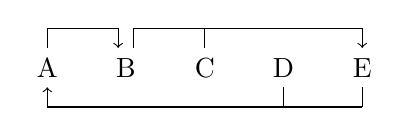
\begin{tikzpicture}
    \node (A) at (0,0) {A};
    \node (B) at (1,0) {B};
    \node (C) at (2,0) {C};
    \node (D) at (3,0) {D};
    \node (E) at (4,0) {E};

    \draw[-] (A) -- (0,0.5);
    \draw[-] (0,0.5) -- (0.9,0.5);
    \draw[->] (0.9,0.5) -- (0.9,0.25);

    \draw[-] (1.1,0.25) -- (1.1,0.5);
    \draw[-] (C) -- (2,0.5);
    \draw[-] (1.1, 0.5) -- (4, 0.5);
    \draw[->] (4, 0.5) -- (4,0.25);

    \draw[-] (E) -- (4, -0.5);
    \draw[-] (D) -- (3, -0.5);
    \draw[-] (4,-0.5) -- (0, -0.5);
    \draw[->] (0,-0.5) -- (0, -0.25);
\end{tikzpicture}
\end{figure}
\ppart{1}
List all keys for R

We can see that $A\rightarrow B$ which means we can rewrite the relationships as
$ACDE$. Giving us

\begin{figure}[ht!]
    \center
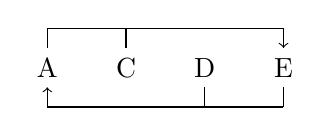
\begin{tikzpicture}
    \node (A) at (0,0) {A};
    \node (C) at (1,0) {C};
    \node (D) at (2,0) {D};
    \node (E) at (3,0) {E};

    \draw[-] (A) -- (0,0.5);
    \draw[-] (C) -- (1,0.5);
    \draw[-] (0, 0.5) -- (3, 0.5);
    \draw[->] (3, 0.5) -- (3,0.25);

    \draw[-] (E) -- (3, -0.5);
    \draw[-] (D) -- (2, -0.5);
    \draw[-] (3,-0.5) -- (0, -0.5);
    \draw[->] (0,-0.5) -- (0, -0.25);
\end{tikzpicture}
\end{figure}

With $A$ and $C$ we are given $E$. Thus we have

\begin{figure}[ht!]
    \center
\begin{tikzpicture}
    \node (A) at (0,0) {A};
    \node (C) at (1,0) {C};
    \node (D) at (2,0) {D};
\end{tikzpicture}
\end{figure}

And we no longer have any relationships.

Similarly we can get the other keys. Giving us the answer:

$ACD$, $BCD$, $CDE$

\ppart{2}
Is R in 3NF?

\part{3}
Is R in BCNF?

\problem{19.6}

\end{document}
